
\documentclass[12pt]{article}
\usepackage{graphicx} % for including images
\usepackage{hyperref} % for creating hyperlinks
\usepackage{amsmath} % for mathematical expressions
\usepackage{lipsum} % for generating dummy text
\usepackage{listings} % for code blocks

\lstset{
  language=bash,
  basicstyle=\ttfamily,
  breaklines=true
}

\begin{document}
% Title page information
\title{Raspberry Pi 4 Environment Configuration}
\author{Jaidon Lybbert, University of Washington}
\date{January 24, 2024}

% Generate the title page
\maketitle

% Abstract section
\begin{abstract}
This report documents the setup and configuration of a portable development environment for a headless Raspberry Pi 4 on a cellular hotspot. The environment consists of a Windows 10 laptop, iPhone 13 Pro, and Raspberry Pi 4B. The Pi is pre-configured with the SSID and password to connect to the iPhone hotspot, and accessed from the laptop through SSH. The Pi is set up with the Neovim editor for on-device development, with language support for Python, Rust, C, C++, and Zig. For debugger support, the Windows laptop is set up with Visual Studio and VSCode with extensions for the same languages.
\end{abstract}

% Introduction section
\section{Introduction}
This document is organized as follows. In Section \ref{sec:background} I describe my experience with embedded systems and software, motivations and intent, and take a look at the physical interface to the Raspberry Pi 4. I devise a plan for setting up my preffered environment in Section \ref{sec:methods}, describe what the actual environment ends up looking like in Section \ref{sec:results}, and discuss the failures and hurdles I faced in Section \ref{sec:discussion}. I conclude in \ref{sec:conclusion} by discussing the improvements I would like to make in the future.

% Methods section
\section{Background}\label{sec:background}
\subsection{Programming Experience}
I graduated with my BS in Electrical Engineering at Eastern Washington University in 2022, with a concentration in Embedded Systems. As part of my coursework, I programmed an FPGA in VHDL to implement a processor supporting a subset of the MIPS instruction set. I did several small projects using the TI ARM\textregistered{} Cortex\textregistered-M4F Based TM4C123G LaunchPad\texttrademark{} MCU evaluation board \cite{ti_ek_tm4c123gxl}, and was introduced to real-time operating systems using the Arduino Mega which I used to make a kitchen timer\cite{lybbert2023} with polling and pre-emptive scheduling.

While at EWU, I was an officer in the IEEE Student Chapter, and made a controller for a skittle-sorting machine, again using the TM4C123G \cite{sorter_project}. 

For two years, I worked at an aerospace startup developing real-time control software for a pressurized gas system using an Allen-Bradley PLC. 

I spent the summer of 2022 doing an internship at SpaceX, where I developed tools in Python to automate workflows and manage parts data.

My graduate studies have been in high-performance parallel computing on the NVIDIA Cuda platform, with some graphics programming in OpenGL and Vulkan, and some deep neural networks. My most recent work has been developing a parallel QR decomposition algorithm with Amazon Lab126 for in-home robotics applications\cite{mixed_precision}.
\subsection{Experience with the Raspberry Pi}
I have done some projects with the Raspberry Pi 3B, and Raspberry Pi-ZeroW. For a time, I had the Raspberry Pi 3B set up as an ad-blocking DNS server using the Pi-hole project \cite{pihole}, and I used the ZeroW for a weather station project as an undergrad in IEEE \cite{weatherstation}.
\subsection{Motivation}
My experience with bare-metal programming and parallel programming on GPUs has given me a great appreciation for on-device debuggers, and memory management. My recent interests have been in programming languages themselves, and the tradeoffs they offer. At the same time, I have been becoming more mobile, and work in a variety of places from my laptop, leaving the desktop, two monitors, and mouse at home. The single low-res screen and trackpad have led me down the path of keyboard shortcuts, macros, and Neovim to ergonomically switch between windows and edit code without using the trackpad. 

These motivations form the basis of the requirements for my development environment (plus version control as a given). 

\begin{itemize}
  \item Portability
  \item Version control
  \item Support for several languages
  \item On-device debugging
  \item Compatibility with Neovim
\end{itemize}


\section{Methods}\label{sec:methods}

\subsection{Installation}
The Raspberry Pi 4B is a relatively simple device to setup following the documentation \cite{raspberrypi_config}. I used a 16GB SD card and flashed the 64-Bit Raspberry Pi OS "Bookworm" to it on my Windows 10 laptop with the provided Raspberry Pi Imager tool. I took a screenshot of the hostname and username configuration, so I wouldn't forget it.

\subsection{Portability}
In advanced settings in the Imager tool, the pre-configured WiFi network was automatically filled, along with the public SSH key from my laptop. I changed the SSID and password for the WiFi network to my iPhone hotspot so I have the option to physically bring my Pi with me and connect with SSH. 

\begin{figure}[h]
\centering
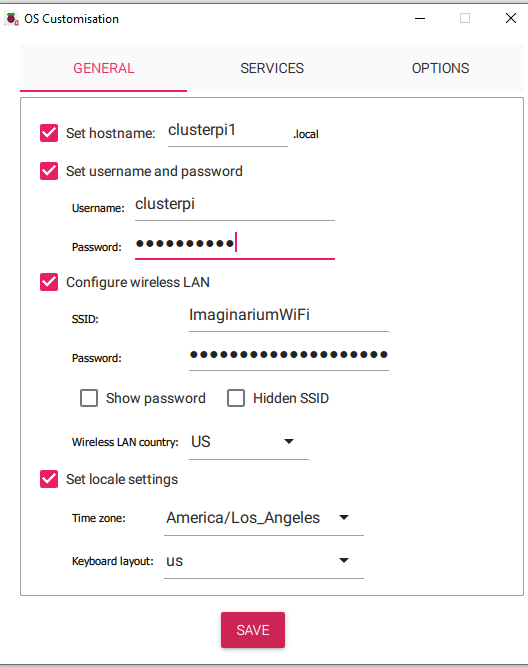
\includegraphics[width=0.75\textwidth]{raspiconfig.png} % replace with your own image file
\caption{The Raspberry Pi Imager showing hostname and username configuration.}
\label{fig:raspiconfig}
\end{figure}

The Pi connected to the hotspot on boot without issue, and I was able to SSH into it by the hostname. I immediately scanned for my home WiFi network, and added it with higher priority using the Network Manager CLI. Switching networks caused the SSH session to hang, but switching networks on my laptop and restarting the SSH connection went without issue.

\begin{figure}[h]
\centering
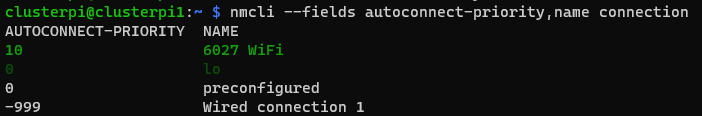
\includegraphics[width=1.0\textwidth]{network-config.png} % replace with your own image file
\caption{WiFi network prioritization in Network Manager. The mobile hotspot was labeled "preconfigured" by default, the home network is named by the SSID "6027 WiFi".}
\label{fig:networkpriority}
\end{figure}

I updated the Pi with APT through my home network. 

\subsection{Version Control}

Once my packages were up to date, I generated an SSH key pair with \verb|ssh-keygen| and copied the public key to my personal Github account. I created a new repository \cite{lybbert2024classwork} and cloned it to the Raspberry Pi. 

\subsection{Language Support}

At this point I checked the remaining space on my SD card with the \verb|df -H| command. I would keep an eye on it as I began installing packages.

\begin{figure}[h]
\centering
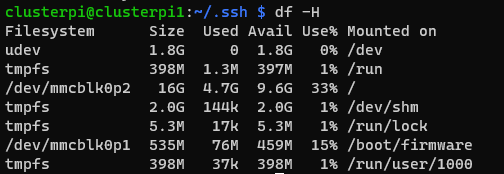
\includegraphics[width=1.0\textwidth]{freespace.png} % replace with your own image file
\caption{Free space on the SD card after basic installation. The filesystem has ~9GB available.}
\label{fig:freespace}
\end{figure}

The full set of languages I want to support are:
\begin{itemize}
  \item Python
  \item Rust
  \item C
  \item Zig
  \item C++
\end{itemize}

I found GCC and Python came pre-installed with the OS. 
I installed Rust by fetching and executing the installer with the one-liner 
\begin{lstlisting}
curl --proto '=https' --tlsv1.2 -sSf https://sh.rustup.rs | sh
\end{lstlisting}
as suggested by the docs \cite{rust_installation}.

I compiled Zig from source using the zig-bootstrap \cite{zig-bootstrap} repository, since it seemed like the right thing to do. The only dependency missing to compile Zig was CMAKE, which I planned to install anyway. I installed Ninja as well to speed up the build process.

I got the triplet for the raspberry pi using

gcc -dumpmachine

I set the CMAKE environment variable to use Ninja instead of Make.

export CMAKE_GENERATOR=Ninja

Then ran the build script for Zig

./build aarch64-linux-gnu native

It occured to me as the build spooled up that this was the first real workload I put on the device. I gave the small adhesive heatsink I put on the SoC an ill-advised finger test and determined it was getting spicy. As it turns out the Pi is quite slow relative to the size of the job of compiling Zig. It would take several hours, though I went to sleep and don't know exactly how long. After looking at the repository again, I realized that I wasn't just compiling Zig, I was also compiling LLVM, LLD, Clang, zlib, and zstd. 

A development environment is set up on the device using Neovim with language support for Python, Rust, C, C++, and Zig. By default, Neovim supports syntax highlighting for these languages, for code completion and static analysis, language-specific plugins are added. A VSCode-based development environment is set up on the Windows 10 machine for instances when a debugger is necessary, with extensions for Python, Rust, and Zig. Visual Studio is used for C and C++, since those projects are built with MSBuild through CMAKE, which outputs Visual Studio projects. Git is installed on both machines for version control.

% Results section
\section{Results}\label{sec:results}
I initially tried installing the Raspberry Pi OS using the same method I had used for the Raspberry Pi 3B several years ago. It used to be the case that you could pre-configure the WiFi connection by flashing the image to the SD card, then copying a \verb|wpa_supplicant.conf| file to the boot partition before installing it to the device. This is no longer supported by the "Bookworm" Raspbery Pi OS and onwards \cite{raspberrypi_config}. 

% Discussion section
\section{Discussion}\label{sec:discussion}
\lipsum[8-9] % replace with your own text

% Conclusion section
\section{Conclusion}\label{sec:conclusion}
\lipsum[10] % replace with your own text

% Bibliography from refs.bib
\bibliographystyle{plain}
\bibliography{refs}

% Acknowledgments section
\section{Acknowledgments}
\lipsum[11] % replace with your own text

% Appendices section
\appendix
\section{Appendix A}
\lipsum[12] % replace with your own text

\section{Appendix B}
\lipsum[13] % replace with your own text

% Figures and tables section
\section{Figures and Tables}
% Example of including a figure
\begin{figure}[h]
\centering

\includegraphics[width=0.5\textwidth]{ferris_the_crab.png} % replace with your own image file
\caption{Example of a figure caption}
\label{fig:example}
\end{figure}

% Example of creating a table
\begin{table}[h]
\centering
\begin{tabular}{|c|c|c|}
\hline
A & B & C \\ \hline
1 & 2 & 3 \\ \hline
4 & 5 & 6 \\ \hline
\end{tabular}
\caption{Example of a table caption}
\label{tab:example}
\end{table}

\end{document}
